\section*{Chronologie}\addcontentsline{toc}{section}{Chronologie}
\fancyhead[RO]{Chronologie}
% \fancyhead[LO]{}

    Die \ceva{c-base} ist eine abgestürzte Raumstation unter Berlin, die sich seit 1995 rekonstruiert~\cite{cbasebook}, ein als \cevain{cbrp} - \cevain{c-base reconstruction project, cbrp} bekannter Prozess. Folgende Epochen lassen sich unterscheiden~\cite{cbasepressemap}~\cite{cbasebook}:
    % \twofonts{
    \begin{enumerate}
        \item \textbf{Unzeit:} vor -4,5 Milliarden Jahre, identisch mit der \textbf{Fernen Zukunft:} ursprüngliche bzw. zukünftige Konstruktion der \ceva{c-base}.
        
        \item \textbf{Urzeit: } -4,5 Milliarden Jahre (Absturz) bis -100.000 Jahren (eigenständiges Einschalten des Bordcomputers \cevain{c-beam} \cite{cbasepressemap}.
        
        \item \textbf{Keimzeit:} -100.000 Jahre bis ca. 1965 (Sichtbarwerdeung der Antenne). Erste Schritte der Selbstrekonstruktion. 
        
        \item \textbf{Vorzeit:} ca. 1965 bis 1995 (Auffindung des \cevain{urartefacts}). Erste Inspiration von Karboneinheiten durch \ceva{c-beam}. Vorschriftliche Periode. Mythische Periode; Erste Zusammenkünfte der \cevain{gründer} (\cref{tab:gruender}).
        
        \item \textbf{Archaische Zeit:} \cevain{cbrp1}.  Februar 1995 -- Mai 2000 Oranienburger Str. 2.  Nachbau und Rekonstruktion einer Schleusensektion auf 270$m^2$ \cite{cbasepressemap}~\cite{cbasebook}. Heldenzeit.
        
        \item \textbf{Frühzeit:} - \cevain{cbrp2}.   Juni 2000 -- August 2002 Rungestr. 20.  Nachbau und Rekonstruktion der Multimodulstation \cevain{RS20} auf 524$m^2$.~\cite{cbasepressemap}~\cite{cbasebook} 
        
        \item \textbf{Zwischenzeit:} \cevain{cwischendecc}.  September 2002 -- Juli 2003 Franz-Mehring-Platz Nr. 1. 
        Auslagerung wegen Wartungsarbeiten in der \ceva{RS20}.~\cite{cbasepressemap}~\cite{cbasebook} 
        
        \item \textbf{Mittelalter:}  \cevain{cbrp3a}. August 2003 -- ca. 2015 (Erscheinen des \ceva{c-booc}). Rungestr. 20. 
         Erweiterung der Fläche auf ca. 720$m^2$ auf 2 Etagen. Fortgesetzte Konstuktion. \cite{cbasepressemap}~\cite{cbasebook} 
        
         \item \textbf{Neuzeit:} \cevain{cbrp3b}. 2015 -- heute. Verfeinerung und Dekadenz. Verinnerlichung, Selbstbewusstwerdung. Mission und Ausgründungen.
    \end{enumerate}
    % }

Eine Überblick über die Dauer der einzelnen Perioden gibt \cref{fig:perioden}.

\begin{figure}
    \centering
        \documentclass{standalone}
\usepackage{tikz}
\usepackage{fontspec}

\newcommand{\ceva}[1]{ {\fontspec{[ceva-c2.ttf]}#1}}
\newcommand{\cevain}[1]{ {\fontspec{[ceva-c2.ttf]}#1} | \emph{#1}}

\begin{document}
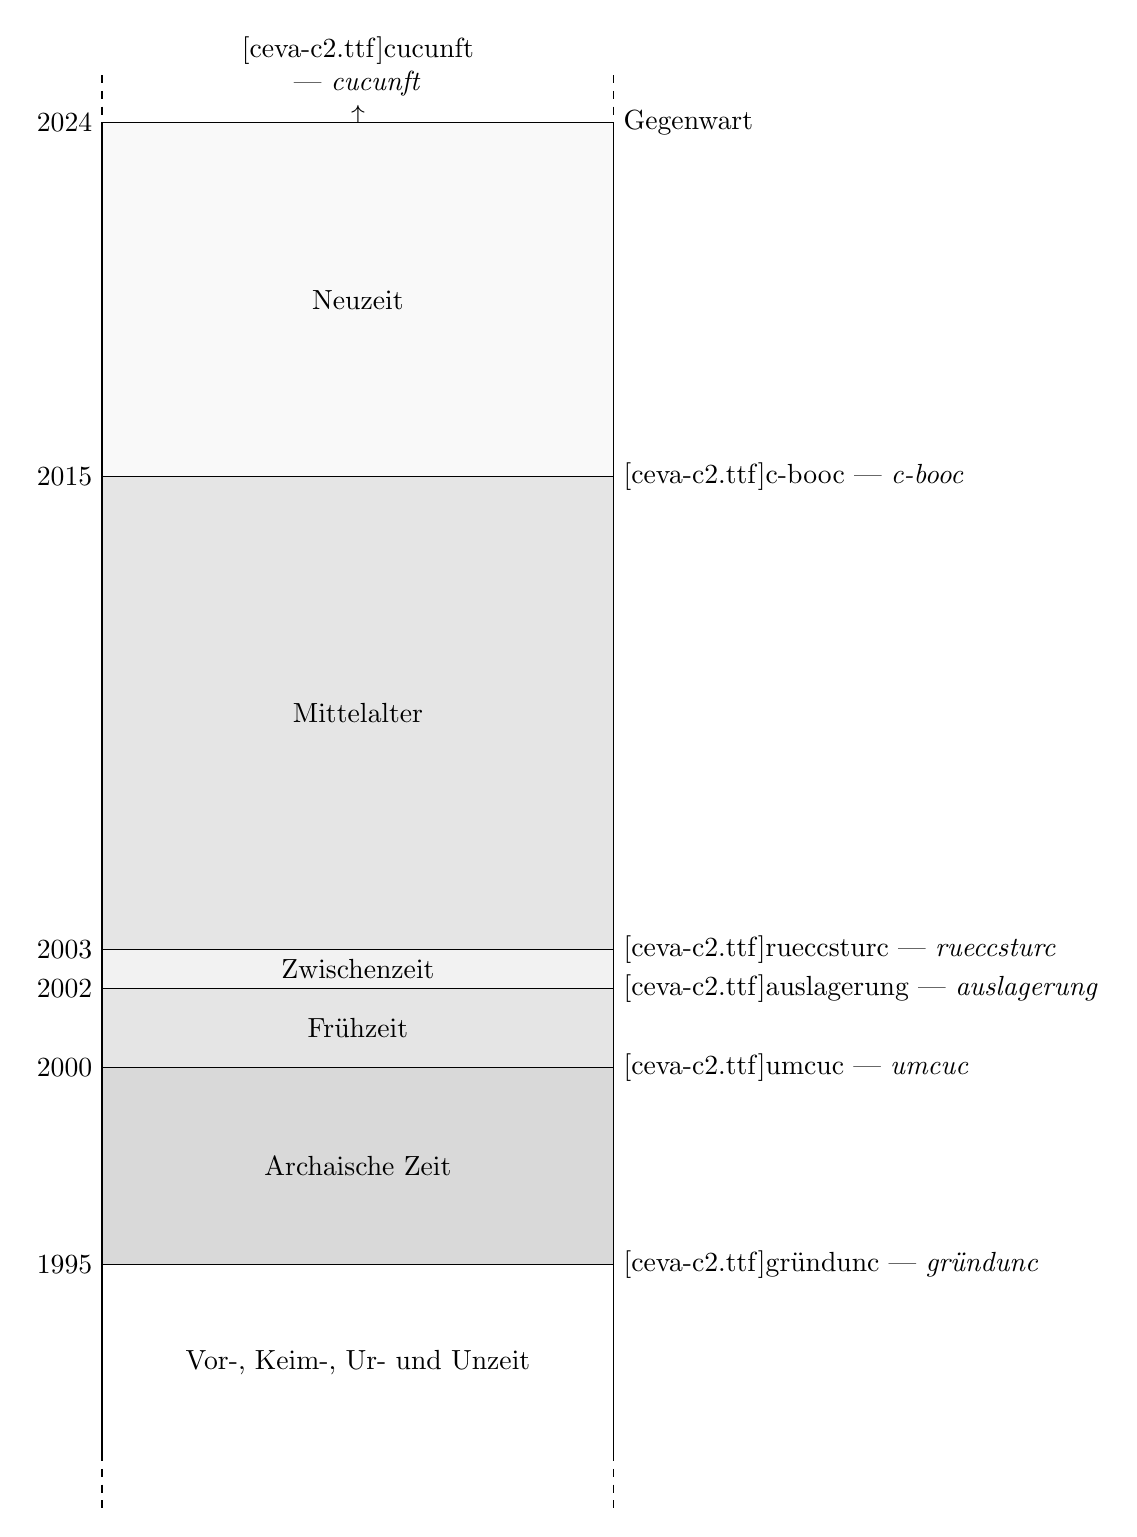
\begin{tikzpicture}[yscale=0.5,xscale=1.3]
    % \draw (0) rectangle (0,,1);
    \foreach \i in {124.4,124.8,125.2} 
        {
        \draw (0,\i) -- (0,\i-0.2);
        \draw (5,\i) -- (5,\i-0.2);
        }

    \node at (2.5,125) {\parbox{20ex}{\centering\cevain{cucunft}\\ $\uparrow$ }};
    
    \node [right] at (5,124) {Gegenwart};
    
    \draw[fill=gray!5] (0,124) node [left] {2024} rectangle node {Neuzeit} (5,115) node [right] {\cevain{c-booc}};
    % \draw (0,115) -- (0,124); draw (5,114) -- (5,124); \draw (0,115
    
    \draw[fill=gray!20] (0,115) node [left] {2015} rectangle node {Mittelalter} (5,103) node [right] {\cevain{rueccsturc}};
    
    \draw[fill=gray!10] (0,103)  node [left] {2003} rectangle node {Zwischenzeit} (5,102) node [right] {\cevain{auslagerung}};
    
    \draw[fill=gray!20] (0,102)  node [left] {2002} rectangle node {Frühzeit} (5,100) node [right] {\cevain{umcuc}};
    
    \draw[fill=gray!30] (0,100)  node [left] {2000} rectangle node {Archaische Zeit} (5,95) node [right] {\cevain{gründunc}};
    % \node at (0,95) [left] {1995};
    
    \draw[draw=none] (0,95)  node [left] {1995} rectangle node {Vor-, Keim-, Ur- und Unzeit} (5,90) ;
    \draw (0,95) -- (0,90); \draw (5,95) -- (5,90);
    
    \foreach \i in {89.8,89.4,89} 
        {
        \draw (0,\i) -- (0,\i-0.2);
        \draw (5,\i) -- (5,\i-0.2);
        }
    
    
    % \draw[<->] (0,95) rectangle (0,65);
\end{tikzpicture}

\end{document}

    \caption{Periodisierung der Rekonstruktionsgeschichte}
    \label{fig:perioden}
\end{figure}

Der rezente Zustand und Befund ihrer Vorzeit sowie Zukunft ist vor allem in \cite{cbasebook} beschrieben, aber auch in weiteren Veröffentlichungen wie etwa \cite{cbasewebsite}. Der aktuelle Rekonstruktionsstand lässt sich von Ort besichtigen. Im Folgenden werten wir die vorhandenen historischen (schriftlichen) Quellen  aus. Diese stammen überwiegend aus der Frühen Neuzeit mit deutlichen Wurzeln in früheren (bzw. späteren) Zeitaltern.

\begin{table}[ht!]
    \centering
    \begin{tabular}{r|l}
    % \cevain{
    \toprule
        \ceva{cynk}& \emph{cynk} \\
        \ceva{mars}& \emph{mars} \\
        \ceva{nomax}& \emph{nomax } \\
        \ceva{hein-c}& \emph{hein-c } \\
        \ceva{biafra}& \emph{biafra} \\
        \ceva{c\_ana}& \emph{c\_ana} \\
        \ceva{lester}& \emph{lester} \\
        \ceva{antenne}& \emph{antenne} \\
        \ceva{tmf powersau}& \emph{tmf powersau} \\
        \ceva{mash}& \emph{mash} \\
        \ceva{westcar}& \emph{westcar} \\
        \ceva{alex}& \emph{alex} \\
        \ceva{olli}& \emph{olli} \\
        \ceva{wallner}& \emph{wallner} \\
        \ceva{gerhard}& \emph{gerhard} \\
         % \cevain{cynk}\\ \cevain{mars}\\  \cevain{nomax}\\  \cevain{hein-c}\\  \cevain{biafra}\\  \cevain{c\_ana}\\  \cevain{lester}\\  \cevain{antenne}\\  \cevain{tmf powersau}\\  \cevain{mash}\\  \cevain{westcar}\\  \cevain{alex}\\  \cevain{olli}\\  \cevain{wallner}\\  \cevain{gerhard}\\
    \bottomrule
    % }
    \end{tabular}
    
    \caption{Die \cevain{gründer}}
    \label{tab:gruender}
\end{table}

% Da wir hier eine Quellenanalyse 

